\subsection{Sewing threads for backpacks} \label{sec:sewing-thread}

When it comes to choosing your thread, there is of course no right or wrong choice. But there are a few things to consider, and then, there is experimentation, trial and error.

For outdoor applications, and more specifically backpacks, you obviously want to consider the absolute tensile strength of your sewing thread so your seams can live through some abuse, but it is by far not the only criteria. Resistance to ultraviolet light, exposure to water (fresh water as well as sea water) and ability to stretch are amongst the important factors. Personally, I also consider how easy it will be to sew with a particular thread, which is mostly defined by the thread size and quality together with the choice of needle.

\begin{note}
  The choice of needle is not random either, I wanted easy-to-find, universal needles which can easily work through multiple layers of tightly woven and/or coated fabrics. Anything below 90/14 tends to break or bend a little too often for my taste. But I can buy a box of 90/14 or 100/16 all purpose needles anywhere.
\end{note}

Most of the common-man's threads will be either Nylon or Polyester, woven in various ways, advertising various qualities. One can also find higher quality - higher price - threads like PTFE, Dyneema, Kevlar and more but I think this would be beyond the point of building your own pack at home (and these would most likely outlast most fabrics you would use anyway).

\begin{figure}[H]
  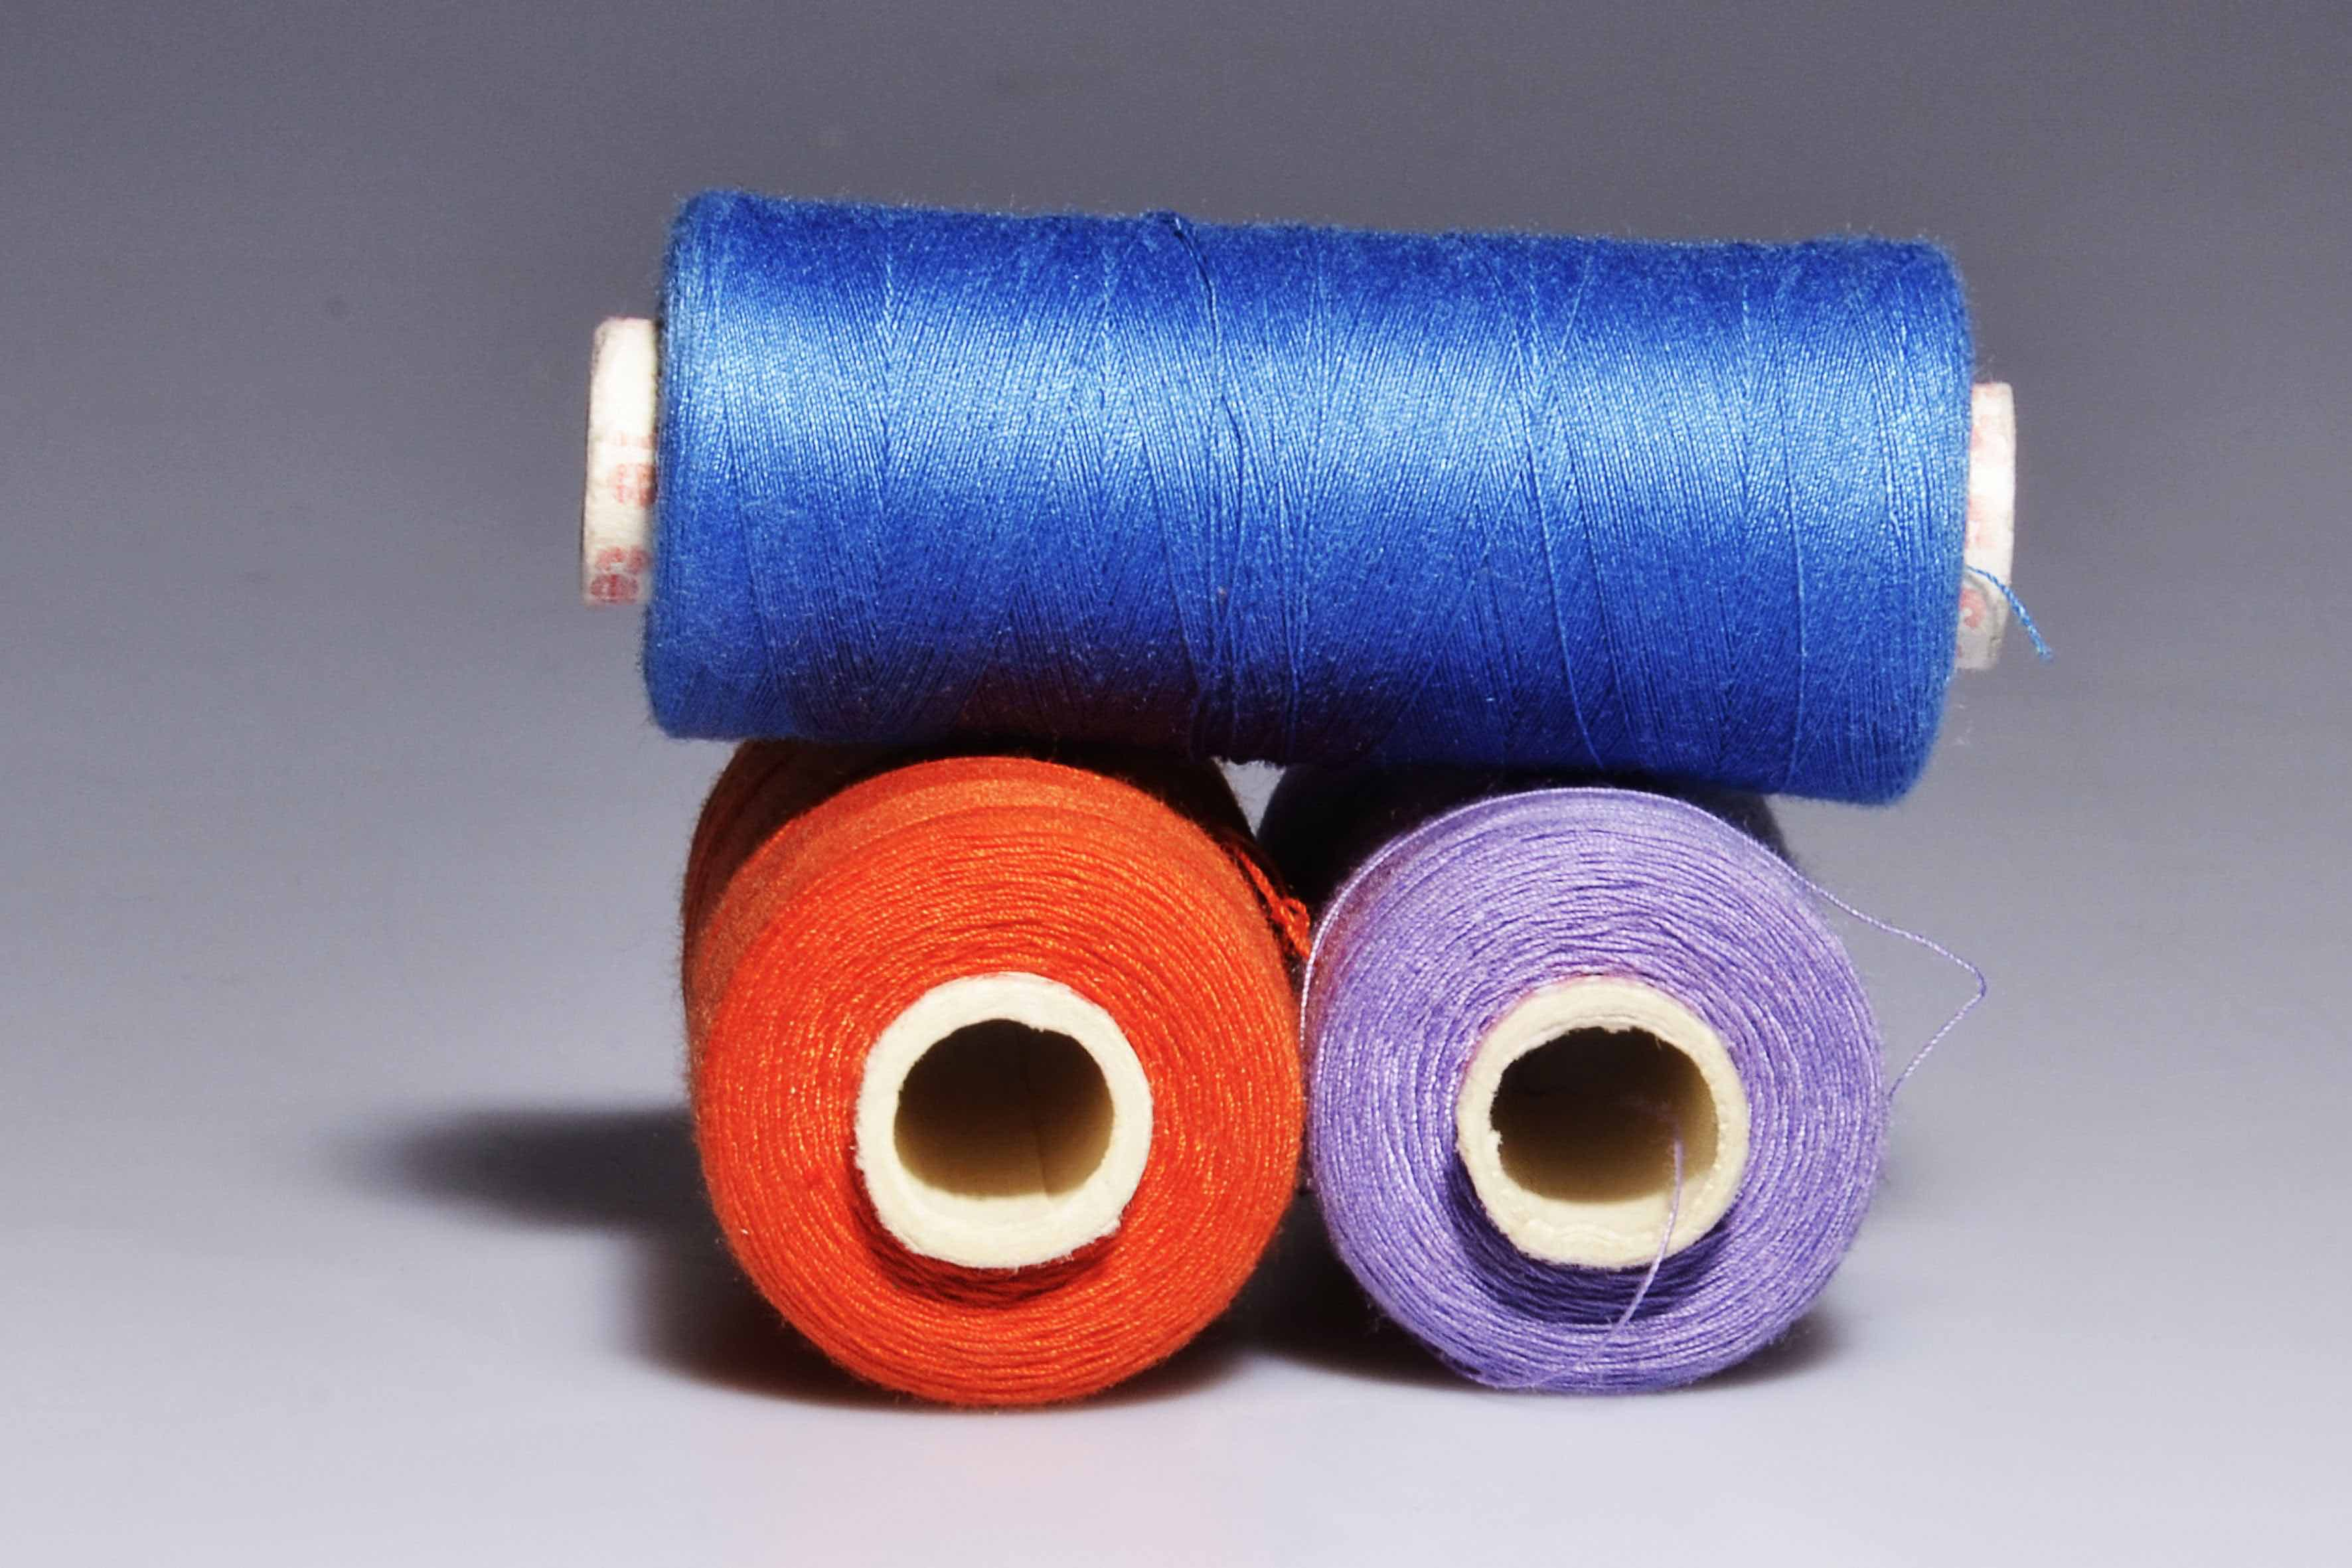
\includegraphics[width=\textwidth]{media/images/place-holder}
  \caption{Illustration of multiple sewing threads}
  \label{img:sewing-threads}
\end{figure}

If only for its resistance to UV exposure, Polyester is the way to go. It is very durable and also offers a very good tensile strength for relatively thin threads. As to the thread size, I always prefer triple stitching a thinner thread than having to deal with a cumbersome heavy thread and beefier needles. It allows a higher combined strength than a heavier single-stitched thread, and allows the fabric under load to stretch together with the tread without tearing the seams. The section \ref{sec:stitching-for-abuse} will provide more details on how I use such thin threads.

Unfortunately, as there is no universal unit - or any proper conversion system - for thread thickness, I can only give you a tensile strength recommendation and which needle size I use for this particular thread. I use a good quality German-made 100\% polyester thread from Alterfil (the S-100) with a tensile strength of 1570 cN (3.5 pounds of force) with 19\% elongation which is around half the single-stitch tensile strength recommended for a backpack seam ( approx. 3000 cN or 6.7 lbf). The S-100 is working perfectly with a size 90/14 or 100/16 universal needle on all fabrics I've tried.

\begin{table}[H]
  \centering
  \begin{tabular}{ | l | l | p{8cm} | }
    \hline
      \textbf{Thread} &
      \textbf{Tensile Strength} &
      \textbf{Recommended use} \\
    \hline
      S-120 &
      1230 cN / 2.76 lbf &
      sports jackets, waistcoats, trousers, coats, jackets, shirts, dresses, sportswear, fabrics of micro-fibre, blouses, underwear/linen, home textiles, curtains, ... \\
    \hline
      S-100 &
      1570 cN / 3.52 lbf &
      outer-wear, sport jackets, waistcoats, trousers, coats, fabrics of micro-fibre, quilting machines \\
    \hline
      S-80 &
      2100 cN / 4.72 lbf &
      jeanswear, sportswear, quilted ornaments, working clothes \\
    \hline
      S-50 &
      3200 cN / 7.19 lbf &
      jeanswear, sportswear, quilted ornaments, working clothes, leather, \textit{rucksacks}, sleeping bags, mattresses, upholstery, hand- and travelling bags \\
    \hline
      S-35 &
      4000 cN / 8.99 lbf &
      jeanswear, quilted ornaments, sportswear, upholstery, \textit{rucksacks} \\
    \hline
  \end{tabular}
  \caption{Alterfil's polyester sewing thread tensile strength recommended use}
\end{table}


Make sure you get yourself a high quality sewing thread, it will be worth every cent. Lower quality threads will probably be enough to hold the seams together (decent tensile strength) but sewing with them will soon become a nightmare. The main issue I have with lower quality products is the uneven weaving of the filaments that can leave bulges and notches along the thread. These imperfections will catch on anything they can on your sewing machine and fabrics, and the thread might tear for no reason. Plus, I find using high quality thread much more forgiving when used with a sewing machine on which the tension is not perfectly calibrated.

\subsection{Stitching for abuse} \label{sec:stitching-for-abuse}

I find it cumbersome to use a heavy-duty thread when sewing together a backpack. Parts of the pack which involve stitching together multiple layers of fabrics can sometime be quite tough on my sewing machine if the needle combined with the thread make for a wide diameter to punch through. So I use a thinner thread instead (see \ref{sec:sewing-thread}).

In combination with this, I use a special stitch, often referred to as the triple stretch stitch or backstitch, which is very robust yet flexible but still uses a single thread and a single needle. The result is much stronger than the tensile strength of the thread itself, and its construction has the added benefit of rendering a single point of failure almost impossible. As the triple pass (two times forward, one time backward each step) prevents any snapped thread from getting loose, resulting in a catastrophic failure of your seam.

The backstitch also allows a seam to stretch beyond what the thread's would normally offer, resulting in overall less stress on a single thread under heavy loads.
